\documentclass{article}
\usepackage{graphicx} % Required for inserting images
\usepackage{float}

\title{Grafici}
\author{GIUSEPPE CALABRESE}
\date{February 2025}

\begin{document}

\begin{figure}
    \centering
    
\includegraphics[width=0.5\linewidth]{Logo Unicam/unicam.jpg}
    \label{fig:enter-label}
\end{figure}

\centering
{\Large \textbf{Università degli studi di Camerino}     \par
    \vspace{1 cm}
        \Large \textbf{Scuola di Scienze e Tecnologie}  \par
        \Large \textbf{Algoritmi e Strutture dati}      \par
    \vspace{4 cm}
        \Large \textbf{GRAFICI SULLA VALUTAZIONE NUMERICA DELLE PRESTAZIONI} \par
    \vspace{1 cm}
        \Large \textbf{Giuseppe Calabrese (Matricola 122630)}}


\newpage
\vspace*{-2.4 cm}
 % Grafico per numero di confronti per AVLTreeSort
\begin{center}
    \Large \textbf{Numero di confronti per AVLTreeSort}
    \begin{figure}[h]
        \centering
        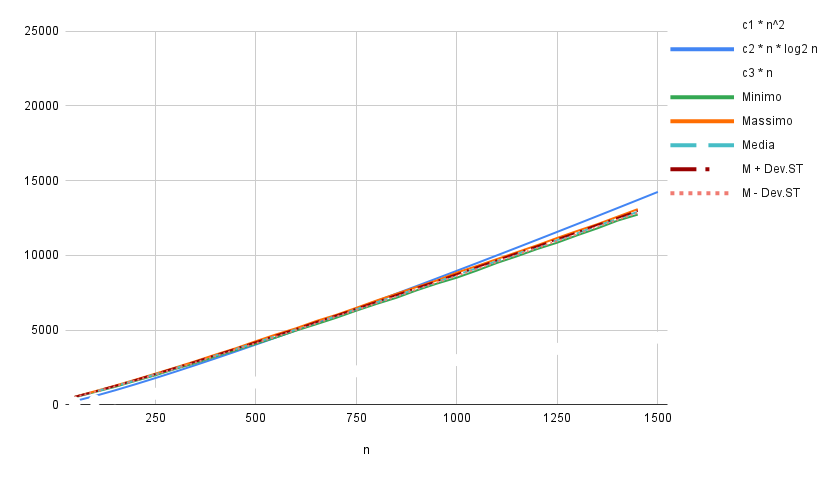
\includegraphics[width=0.98\linewidth]{Grafici/AVLTreeSort.png}
        \label{fig:graph}
    \end{figure}
\end{center}


 % Grafico per numero di confronti per AVLTreeSort
 \vspace*{2.4 cm}
\begin{center}
    \Large \textbf{Numero di confronti per Heap3Sort}
    \begin{figure}[h]
        \centering
        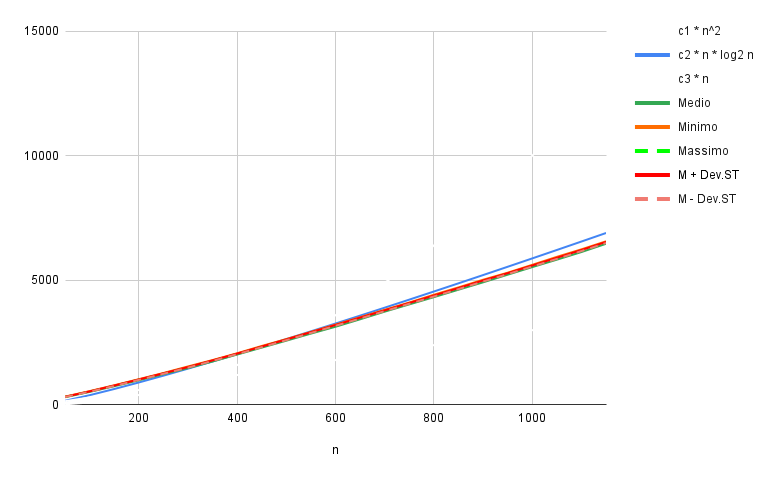
\includegraphics[width=0.97\linewidth]{Grafici/Heap3SortConf.png}
        \label{fig:graph}
    \end{figure}
\end{center}


\newpage
\vspace*{-2.9 cm}
 % Grafico per numero di confronti per AVLTreeSort
\begin{center}
    \Large \textbf{Heap3Sort tempo di esecuzione in ns.}
    \begin{figure}[h]
        \centering
        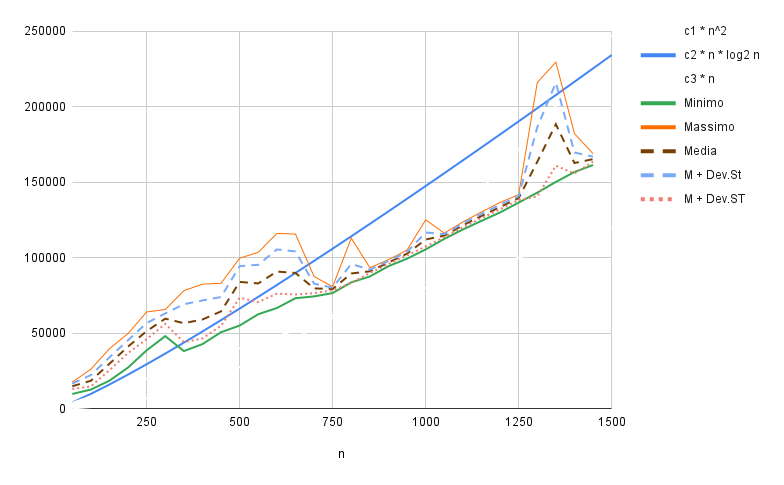
\includegraphics[width=0.95\linewidth]{Grafici/Heap3SortTempNs.png}
        \label{fig:graph}
    \end{figure}
\end{center}


 % Grafico per numero di confronti per AVLTreeSort
 \vspace*{1 cm}
\begin{center}
    \Large \textbf{AVLTreeSort tempo di esecuzione in ns.}
    \begin{figure}[h]
        \centering
        \vspace*{-0.1 cm}
        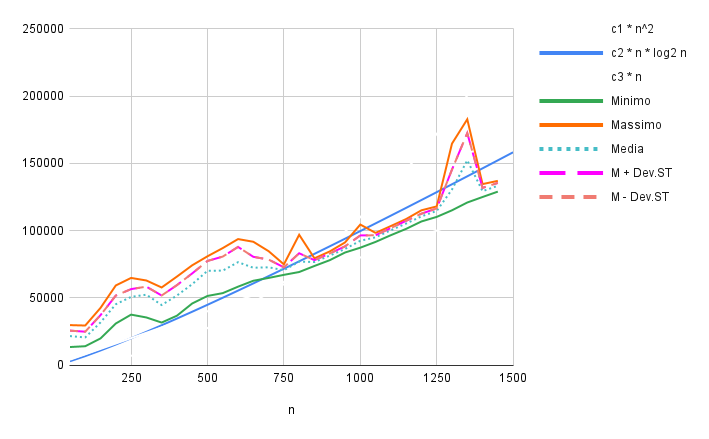
\includegraphics[width=0.95\linewidth]{Grafici/AVLTreeSortTempNs.png}
        \label{fig:graph}
    \end{figure}
\end{center}


\newpage
\vspace*{-2.9 cm}
 % Grafico per Confronto AVL vs Heap caso medio e max per il
 % numero di confronti
\begin{center}
    \Large \textbf{Confronto AVL vs Heap caso medio e max per il numero di confronti}
    \begin{figure}[h]
        \centering
        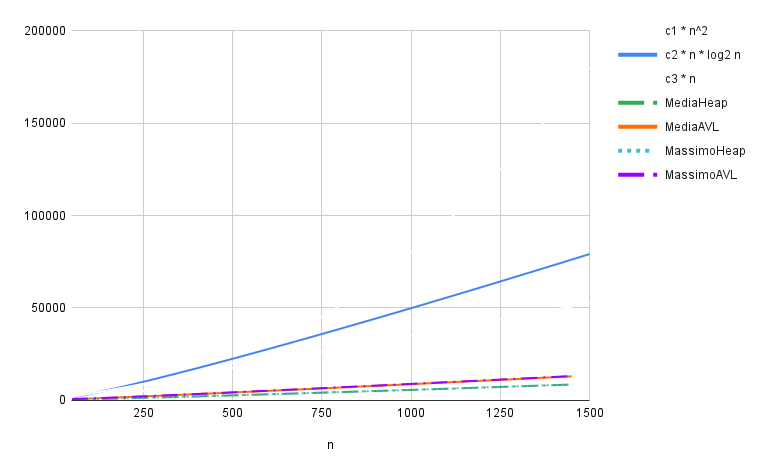
\includegraphics[width=0.95\linewidth]{Grafici/AVLvsHEApNc.png}
        \label{fig:graph}
    \end{figure}
\end{center}


% Grafico per Confronto AVL vs Heap caso medio e max per il
% tempo di esecuzione in ns
 \vspace*{1 cm}
\begin{center}
    \Large \textbf{Confronto AVL vs Heap caso medio e max per il tempo di esecuzione in ns}
    \begin{figure}[h]
        \centering
        \vspace*{-0.1 cm}
        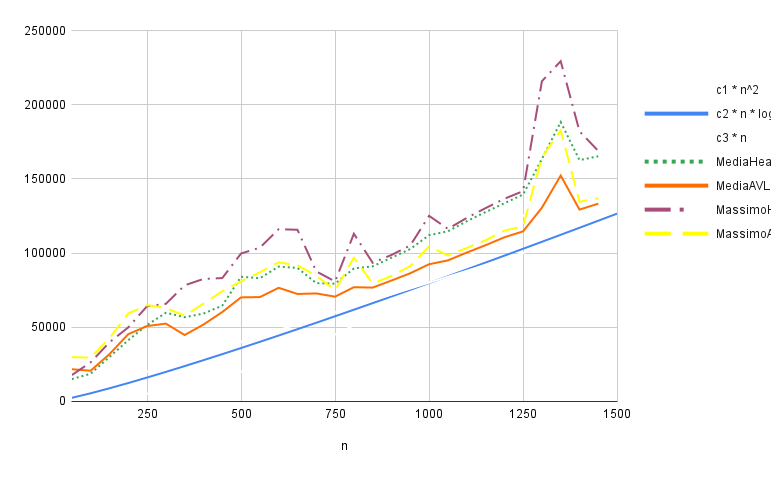
\includegraphics[width=0.95\linewidth]{Grafici/AVLvsHeapTs.png}
        \label{fig:graph}
    \end{figure}
\end{center}

\end{document}